\section{Experiments}
\label{sec:eval}

In this section, we first introduce the dataset and experiment setup,
then present the offline evaluation and give some discussions.
We further give a detailed analysis of proposed problem and model, 
including ablation tests and case study.
Finally, we introduce the online deployment of our model in Taobao and present the results of A/B testing.

\subsection{Datasets}

Inferring e-commerce concepts a user potentially needs is a relatively new problem, 
there is no such public datasets for experiments.
To create large amounts of gold standard data to train our model, 
we collect daily log of our online system, 
where concepts are already integrated in the recommender system. 
In a module called ``Guess What You Like'' at the front page of Taobao app, concepts are displayed as cards to users among the recommended items.
There will be one concept card every ten items on average.
In the snapshot shown in \figref{fig:cloud}(a), concept ``Tools for Baking'' replaces an item and is displayed as a card, with the picture of a representative item.
%\KZ{How do did you get the concept on the taobao page in the first place. 
%It seems that each concept is associated with a set of items on the taobao page.
%If these concepts were created manually, then why not use them as positive
%data directly?}
Once users click on this card, 
it jumps to a page of related items such as egg scrambler and strainer.
In order to alleviate the potential influence of the item picture on users' decision making,
we collect positive samples from those user-concept clicks
only if that user continues to click at least two related items after entering the concept card.
For the same reason, negative samples come from at least two exposes of the same concept (but different item pictures) without any clicks.
We collect samples for continuous four days during January 11 to January 14, 2019, and use the data of first three days for training and validation. 
We randomly select $10\%$ samples of the last day for testing.
The ratio of negative and positive is around $37:1$.
For user-item interaction data, we collect 30-days transaction records on Taobao platform for each user in our data.
Detailed statistics of our dataset is illustrated in \tabref{tab:exp_data}.
\begin{table}[th]
	\centering
	%\scriptsize
	\begin{tabular}{l|c|c|c}
		\hline
		  & Training & Validation & Testing \\
		\hline
		\# of samples & 32,496,827 & 328,251 & 1,237,506 \\
		\# of users & 16,120,600 & 323,544 & 1,121,475 \\
		\# of concepts & 4,760 & 2,935 & 3,176 \\
		\hline
		\# of items & 438M & 76M  & 141M \\
		\# of categories & 15,257 & 11,799 & 14,590 \\
		\# of brands & 1,434,659 & 428,036 & 1,088,480 \\
		\hline
	\end{tabular}
	\caption{Statistics of Taobao's dataset.}
	\label{tab:exp_data}
\end{table}

%The e-commerce concept net we use as the knowledge graph is incomplete at current stage.
%Ideally, all edges between concept and other node should be bi-directional. For example, the relation from a category to a concept is clearly not the same as its reverse. 
%In practice, due to the fact our concept net is still under construction, we only adopt edges from item, category and brand to concept in our experiments.
Based on years of e-commerce experience, we mainly select five meta-paths (\figref{fig:model}) in our experiments: ``\textbf{UIC}'', ``\textbf{UITC}'' and ``\textbf{UIBC}'' for behavior  paths; ``\textbf{UTC}'' and ``\textbf{UBC}'' for preference paths.
Longer paths are not selected since they are likely to bring noises.
%We do not include meta-paths taking concept as intermediate node such as ``\textbf{UCTC}'' for this reason.




\subsection{Experiment Setup}

\noindent
\textbf{Evaluation Metrics}

\noindent
We perform evaluation of different models in two experiment scenarios.
1) In click-through-rate (CTR) prediction, we apply the trained model to each sample of test set and calculate $AUC$ based on the output score to evaluate the overall performance; 2) In top-$N$ recommendation scenario, 
we use the trained model to select $N$ concepts with highest predicted scores for each user in the test set. 
we evaluate the results by Hit Ratio ($HR@N$), and Normalized  Discounted Cumulative Gain ($NDCG@N$),
which are widely used in recommendation tasks having very few ground-truth results \cite{huang2018improving,chen2018sequential}.
In order to make sense under the second scenario, 
we augment the test set mentioned above by removing samples where the user does not have any positive clicks,
and report averaged $HR$ and $NDCG$ across users.

\noindent
\textbf{Baselines}

\noindent
We compare with the following state-of-the-art baselines:
\begin{itemize}
	\itemsep0em
	\item \textbf{BPR} \cite{rendle2009bpr} is the Bayesian Personalized Ranking model that minimize the pairwise ranking loss for implicit feedback.
	\item \textbf{Wide\&Deep} \cite{cheng2016wide} is the widely used recommendation framework, which jointly trains wide linear models and deep neural networks. We use embeddings of users, concepts and other entities to feed Wide\&Deep.
	\item \textbf{MCRec} \cite{hu2018leveraging} is the state-of-the-art HIN based model for recommendation. It treats the KG as HIN and extracts meta-path based features for modeling user-item interaction. 
	We feed e-commerce concept net as the HIN for this baseline.
	\item \textbf{KPRN} \cite{wang2018explainable} is another state-of-the-art knowledge-aware recommendation model, which aims to reason over KG by composing both entities and relations. 
%\KZ{Where is BPR in the results table? I think it is better if you can include
%some results on some standard datasets, rather than just private taobao data.
%Also, I think you need to release the code of all your implementation, including
%the baselines to be more convincing.}
\end{itemize}

\noindent
\textbf{Implementation Details}

\noindent
We implement our model using the python library of TensorFlow \footnote{\url{www.tensorflow.org}}. 
We set the length of user behavior sequence to $15$,
and sampled path instance within each meta-path to at most $50$.
The dimension of entity embeddings (item, concept, category, etc.) is set to $20$, 
and the dimension of output layer is set to $32$,
The hidden state size of GRU is set to $40$.
All parameters are randomly initialized with Gaussian distribution.
We perform a mini-batch log-likelihood loss training with a batch size of $512$ for $5$ training epochs.
We use Adam optimizer \cite{kingma2014adam}, and the learning rate is initialized to $0.001$.
To prevent the gradient explosion problem for training GRU networks,
we set gradient clip-norm as $5$.
For all the comparison models, 
we refer to their original papers and tune the parameters using the validation set as well.
With the help of a powerful distributed TensorFlow machine learning system in Taobao, 
we use $4$ parameter servers and $20$ workers,
and the whole training process can be finished in $4$ hours.

\subsection{Offline Evaluation}
\label{sec:off_eval}

We report the experimental results in \tabref{tab:eval_main} and \figref{fig:topn}.
CptInfer outperforms all the baselines, improving the result by up to 2.4\% in $AUC$.
Improvements in $HR$ and $NDCG$ also reveal the superiority of our model.
BPR and Wide\&Deep perform comparably poorly than other baselines, since they do not incorporate extra knowledge from e-commerce concept net into the model, failing to leverage rich features from paths between users and concepts.
For knowledge-aware baselines, 
%we mainly focus on implementing the encoding of paths in different ways according to the ideas mentioned in their papers respectively.
the main difference is the encoding of paths and attention mechanism.
For fair comparison, 
extra information appeared in our problem such as sequential user behaviors, user profile and concept schema, 
are also fed into all the baselines as well, in a compatible way.
MCRec performs best among all baselines, 
since it also try to characterize a three-way interactions among user, paths and the concept.
CptInfer substantially outperforms MCRec to achieve the best performance,
which indicates the importance of modeling mutual attentive influence of three components simultaneously.
KPRN performs worse than MCRec, since the relation name matters in their problem is relatively trivial in our concept net.
The last two lines of \tabref{tab:eval_main} further demonstrate the effectiveness of our proposed attention module. 
By comparing to a degenerated version of CptInfer, which replaces attention cube with average pooling in each component, 
our full model achieves better performance.
\begin{table}[th]
	\centering
	%\scriptsize
	\begin{tabular}{l|c}
		\hline
		Model &   AUC \\
		\hline
		BPR \cite{rendle2009bpr} &  0.6005 \\
		Wide\&Deep \cite{cheng2016wide} &  0.6137 \\
		MCRec \cite{hu2018leveraging} &  0.6447 \\
		KPRN \cite{wang2018explainable} &  0.6417 \\
		\hline
		CptInfer (\textbf{-} att. cube) &  0.6381   \\
		CptInfer (full) &  \textbf{0.6602} \\
		\hline
	\end{tabular}
	\caption{AUC in CTR prediction on Taobao's dataset.}
	\label{tab:eval_main}
\end{table}

\begin{figure}[th]
	\centering
	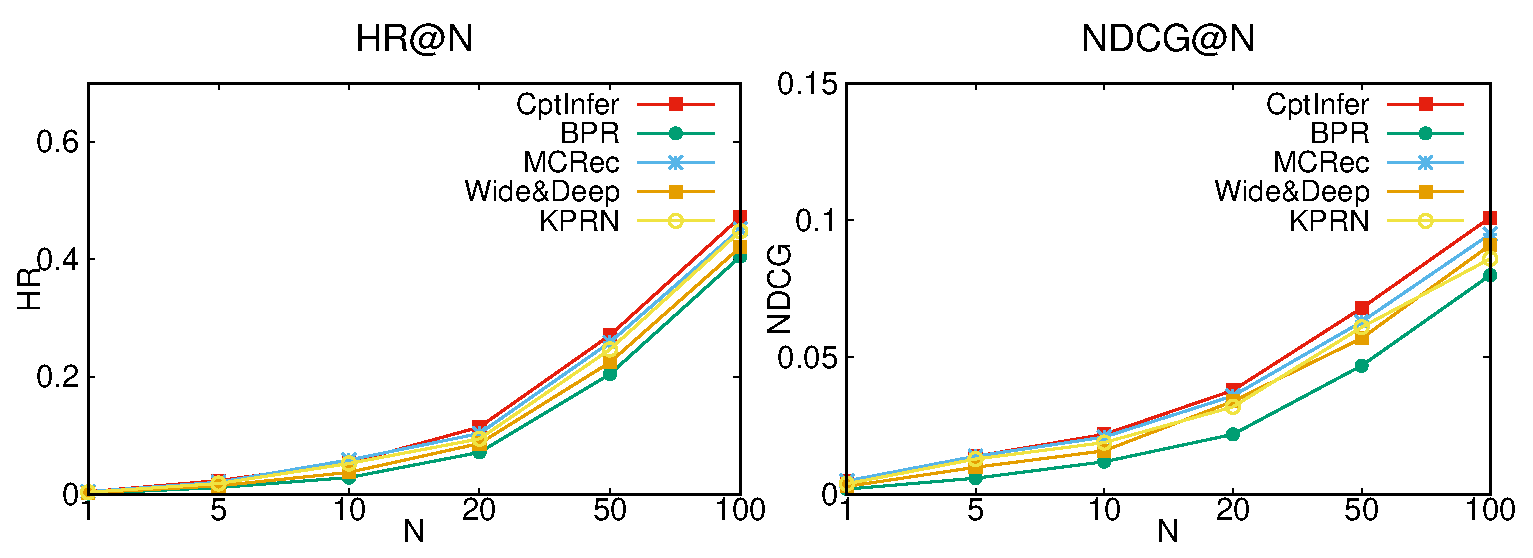
\epsfig{file=figures/topn.eps, width=\columnwidth}
	\caption{HR and NDCG in Top-N recommendation.}
	\label{fig:topn}
\end{figure}



\subsection{Ablation Study}
In this subsection, we explore the contribution of various components of our model.
We report AUC on evaluation set to compare different variations in \tabref{tab:ablation}.


\noindent
\textbf{Behavior Paths vs Preference Paths}

\noindent
We first evaluate how different types of meta-path between users and concepts effect final performance. 
If we remove all paths from CptInfer, AUC drops by $6.8\%$, 
revealing the huge benefits brought by the concept net.
Between behavior paths and preference paths,
we can observe that AUC drops more severely when removing the former ones,
which indicates that behavior paths are more important than preference paths in our model.
It appears that recent clicks or purchases of items play a larger role 
in reflecting user needs than long-term preferences,
which may inflect that user needs are changeable and unstable, and they can be easily influenced.
\begin{table}[th]
	\centering
	%	\scriptsize
	\begin{tabular}{l|c|c}
		\hline
		Variation  & AUC   & Decrease (\%)\\
		\hline
		- behavior paths  &  0.6826 & 4.03\\
		- preference paths  & 0.6934 & 2.41\\
		- all paths & 0.6694 & 6.08\\
		\hline
		\hline
		- user behavior sequence & 0.7010 & 1.30\\
		- user profile & 0.6986 &  1.65\\
		- concept schema & 0.7031 & 1.00\\
		\hline
		\hline
		Full  &  \textbf{0.7101} & 0.0 \\ 
		\hline
	\end{tabular}
	\caption{Ablation tests on validation set.}
	\label{tab:ablation}
\end{table}

\noindent
\textbf{Behavior Sequence vs Side Information}

\noindent
Now we investigate the influence of user behavior sequence and side information in our problem,
where side information further includes user profile and concept schema.
Ablation towards these three components shows that they all contributes to the final inference result, 
while user profile information matters most ($1.65\%$ decrease in AUC).
It is observed that user profile seems more important than user behavior sequence.
The possible reason is that the attention cube degenerates to a matrix, if we remove user profile from the model.
This may lead to a decrease in final performance.



\subsection{Interpretability}
\label{sec:case}

In this part, we give more detailed analysis about the advantages of our proposed model.
A major contribution of CptInfer is that we propose a attention cube to model three-way interactions simultaneously, 
aiming to learn more effective representations for users, concepts and paths.
The attention cube is designed for distinguishing different importances of different factors in an e-commerce interaction, 
which may inspire us to better understand user needs.
Besides the effectiveness shown in \tabref{tab:eval_main} and \figref{fig:topn}, attention cube provides interpretability as well.
Therefore, we analyze the attention values from several perspectives.

In \figref{fig:att}, we visualize average attention weights ${\bm{\alpha_u}}_i$, ${\bm{\alpha_p}}_j$ and ${\bm{\alpha_c}}_k$ for each component of user profile, meta-paths and concept schema.
We can observe that ``\textbf{UIC}'' path has the highest attention weight among all meta-paths, while preference paths ``\textbf{UTC}'' and ``\textbf{UBC}'' are less important.
The result verifies the ablation test towards path variations in \tabref{tab:ablation}.
For aspects of user profile and concept schema, 
it is shown that ``gender'' and ``life stage'' have larger impacts than others,
and the weight of ``kid's life stage'' in user profile is the highest, 
we guess the reason is that a large portion of active users in Taobao are parents who have kids.

\begin{figure}[th]
	\centering
	\epsfig{file=figures/att.eps, width=\columnwidth}
	\caption{Visualization of attention weights for meta-paths, user profile aspects and concept schema aspects. Darker colors indicate higher weights.}
	\label{fig:att}
\end{figure}

We further investigate the attention weights to reveal some interesting findings.
During inference, if the gender of a user matches to the gender of a concept, the attention weights of ``gender'' in both user profile and concept schema become nearly twice larger than not matching.
This indicates our model can explicitly learn rules such as a young female user is more likely to need a concept ``Party for girls'' rather than ``Party for boys''.
To see if the same user has different preferences on meta-paths regarding different concepts, we randomly pick a user in training set as illustrative example shown in \figref{fig:att2}.
The anonymous user has two positive interactions of concept cards: ``Learning to Walk for Kids'' and ``Fishing in River''.
After digging into transaction data,
we find that this user recently clicks a lot of kids related items, resulting high importance of behavior paths shown in his attention distribution when facing concept ``Learning to Walk for Kids''.
On the contrary, he has few behaviors related to fishing. 
Accordingly, the attention weights of preference paths are much higher than average when facing concept ``Fishing in River'' since his long-term category preference is ``fishing equipments''.
Besides, attention weights of ``life stage'' in ``Learning to Walk for Kids'' is higher than ``Fishing in River'' because the former one is constrained to ``teenager'' while the latter has no constraints.
This case demonstrates the interpretability of our proposed model.

\begin{figure}[th]
	\centering
	\epsfig{file=figures/att_2.eps, width=\columnwidth}
	\caption{Visualization of attention weights for an anonymous user. Darker colors indicate higher weights.}
	\label{fig:att2}
\end{figure}

\subsection{Online Testing}

The above offline experimental results have shown superiority of our proposed model.
We deploy it online in Taobao platform to test its practical performance with a standard A/B testing configuration.
The experiments are conducted in the online module introduced in \figref{fig:cloud} (a).
We integrate the inferred user needs for each online user to our recommender system, 
making recommendations of concept cards (one concept plus one representative item).
Two online metrics are used to measure the performance: 
click-through-rate (CTR) and category-discovery (Discovery). Detailed definitions are as follows:
\begin{equation}
CTR = \frac{\# \text{ concept card clicks}}{\# \text{ concept card exposes}},
\end{equation}
\begin{equation}
Discovery = \text{Avg}_u(\frac{\# \text{ new click-categories in 15d}} {\# \text{ click-categories}})
\end{equation}
where Discovery is a measurement of how many distinct categories (of representative items in concept cards) a user clicked today are newly discovered (not clicked in the past $15$ days on Taobao platform).
It is a temporary\footnote{Designing a proper metric to evaluate novelty or serendipity in industry recommendation is a hard and unsolved problem.} metric used in Taobao to evaluate the novelty of recommendation results.

We deploy the proposed CptInfer online and daily update our model.
When recommending a concept card, online recommender system first output a list of items as usual, 
then we pair the items in the list with inferred top concepts, and filter those items which are not related to any concepts. In the meantime, items within top concepts will complement the list.
Followed by a regular ranking module, concept cards with highest scores will then be displayed to users.
Comparing to the former strategy of user needs inference mainly based on FTRL \cite{mcmahan2013ad}, 
online results of A/B testing show that CTR increases by a relative gain of $\textbf{3.7\%}$, 
which indicates that the proposed model infers user needs more accurately. 
On the other hand, Discovery is improved by $\textbf{5.6\%}$, 
showing our model is able to bring more novelty and further improve user satisfaction.

Online prediction time is important to real-world industry systems. 
Comparing to other online deep models, 
the additional time cost of our model mainly lies on the generation of different path instances between the user and the candidate concept.
For efficiency consideration,
we constrain the number of instances for each meta-path to a small number of $5$ in practice. Given a node, we offline filter out all the out-going nodes with a low priority score (mentioned in \secref{sec:path}), and build an alias table.
In this way, the time cost of node sampling is $O(1)$.
Further empowered by a specially optimized graph search engine in Taobao, 
the average running time of user needs inference is $10$ ms, 
which is shorter than following ranking module and can be tolerated by the recommender system.

To further verify the advantage of user-needs driven recommendation, 
we compare recommending a concept card with 
recommending an item (by traditional strategy)
at the same position on ``Guess What You Like''.
Online evaluation shows significant improvements \footnote{This comparison is not entirely fair due to the different display form between a concept card and an item. 
But the large improvements still indicate the potential value of user-needs driven recommendation. Integrating user needs understanding to general item recommendation is included in our future work.} of recommending concept cards:
\textbf{5.3\%} in CTR and \textbf{9.6\%} in Discovery.
If we further consider the purchases of related items in the page guided by concept cards, total sales volume (GMV) is improved by \textbf{84.0\%}, which demonstrates the value and potential of user-needs driven recommendation.









